%=========================================================================
% Start of
%=========================================================================
\preClass{Trigonometric Identities}

\begin{problem}
\item Use the unit circle and the definition of sine and cosine to
  provide a justification for the identity
  \begin{eqnarray*}
    \sin^2(\theta) + \cos^2(\theta) & = & 1.
  \end{eqnarray*}

  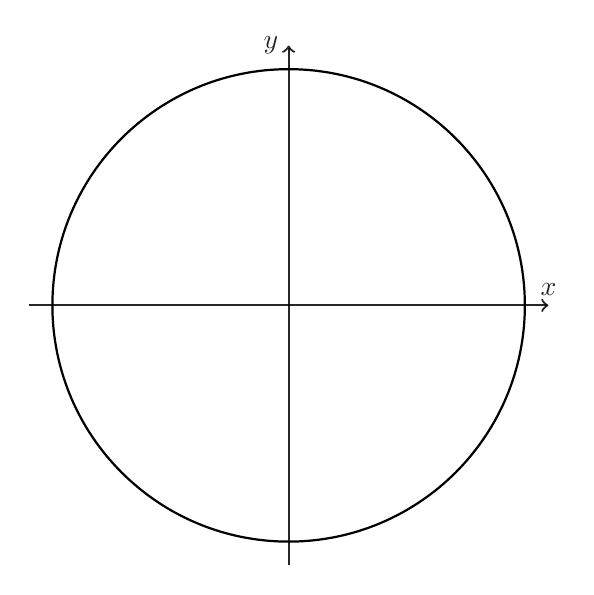
\begin{tikzpicture}[y=3cm, x=3cm,font=\sffamily]
      \draw[thick,opacity=0.85,->] (0, -1.1) -- (0,1.1) node[anchor=east] {$y$};
      \draw[thick,opacity=0.85,->] (-1.1, 0) -- (1.1,0) node[anchor=south] {$x$};
      \draw[thick] (1,0) arc (0:360:1);
%      \draw[thick] (0,0) -- (30:1) node[midway,anchor=south] {$r$}
%          -- ++(-90:0.5) node[midway,anchor=west] {$y$}
%          -- (0,0) node[midway,anchor=north] {$x$};
%      \draw[fill=black] (30:1) circle (0.02);
%      \draw[text=black] (0:0.2) arc (0:30:0.2) node[midway,anchor=west] {$\theta$};
    \end{tikzpicture}

  \sideNote{Choose a point on the circle, draw the associated
    triangle, and then use the appropriate definitions.}

\end{problem}


\actTitle{Trigonometric Identities}
\begin{problem}
\item Is the equation
  \begin{eqnarray*}
    \left( \sec(\theta) - \tan(\theta) \right) \cdot \left(\csc(\theta)+1\right)
    & = &
    \cot(\theta)
  \end{eqnarray*}
  true for all $\theta$? (Fully justify your answer!)

  \vfill

  \clearpage

\item Is the equation
  \begin{eqnarray*}
    \frac{1+\csc(3\beta)}{\sec(3\beta)} - \cot(3\beta) & = & \cos(3\beta)
  \end{eqnarray*}
  true for all $\beta$? (Fully justify your answer!)

  \vfill

  \clearpage

\item Is the equation
  \begin{eqnarray*}
    \cos^2(4\alpha) & = & 1 - \sin^2(4\alpha)
  \end{eqnarray*}
  true for all $\alpha$? (Fully justify your answer!)

  \vfill

  \clearpage

\item Is the equation
  \begin{eqnarray*}
    \tan^2(\theta) + 1 & = & \sec^2(\theta)
  \end{eqnarray*}
  true for all $\theta$? (Fully justify your answer!)

  \vfill

  \clearpage

\end{problem}

\postClass

\begin{problem}
\item Briefly state two ideas from today's class.
  \begin{itemize}
  \item
  \item
  \end{itemize}
\item
  \begin{subproblem}
    \item
  \end{subproblem}
\end{problem}


%%% Local Variables:
%%% mode: latex
%%% TeX-master: "../labManual"
%%% End:
